\documentclass[1p]{elsarticle_modified}
%\bibliographystyle{elsarticle-num}

%\usepackage[colorlinks]{hyperref}
%\usepackage{abbrmath_seonhwa} %\Abb, \Ascr, \Acal ,\Abf, \Afrak
\usepackage{amsfonts}
\usepackage{amssymb}
\usepackage{amsmath}
\usepackage{amsthm}
\usepackage{scalefnt}
\usepackage{amsbsy}
\usepackage{kotex}
\usepackage{caption}
\usepackage{subfig}
\usepackage{color}
\usepackage{graphicx}
\usepackage{xcolor} %% white, black, red, green, blue, cyan, magenta, yellow
\usepackage{float}
\usepackage{setspace}
\usepackage{hyperref}

\usepackage{tikz}
\usetikzlibrary{arrows}

\usepackage{multirow}
\usepackage{array} % fixed length table
\usepackage{hhline}

%%%%%%%%%%%%%%%%%%%%%
\makeatletter
\renewcommand*\env@matrix[1][\arraystretch]{%
	\edef\arraystretch{#1}%
	\hskip -\arraycolsep
	\let\@ifnextchar\new@ifnextchar
	\array{*\c@MaxMatrixCols c}}
\makeatother %https://tex.stackexchange.com/questions/14071/how-can-i-increase-the-line-spacing-in-a-matrix
%%%%%%%%%%%%%%%

\usepackage[normalem]{ulem}

\newcommand{\msout}[1]{\ifmmode\text{\sout{\ensuremath{#1}}}\else\sout{#1}\fi}
%SOURCE: \msout is \stkout macro in https://tex.stackexchange.com/questions/20609/strikeout-in-math-mode

\newcommand{\cancel}[1]{
	\ifmmode
	{\color{red}\msout{#1}}
	\else
	{\color{red}\sout{#1}}
	\fi
}

\newcommand{\add}[1]{
	{\color{blue}\uwave{#1}}
}

\newcommand{\replace}[2]{
	\ifmmode
	{\color{red}\msout{#1}}{\color{blue}\uwave{#2}}
	\else
	{\color{red}\sout{#1}}{\color{blue}\uwave{#2}}
	\fi
}

\newcommand{\Sol}{\mathcal{S}} %segment
\newcommand{\D}{D} %diagram
\newcommand{\A}{\mathcal{A}} %arc


%%%%%%%%%%%%%%%%%%%%%%%%%%%%%5 test

\def\sl{\operatorname{\textup{SL}}(2,\Cbb)}
\def\psl{\operatorname{\textup{PSL}}(2,\Cbb)}
\def\quan{\mkern 1mu \triangleright \mkern 1mu}

\theoremstyle{definition}
\newtheorem{thm}{Theorem}[section]
\newtheorem{prop}[thm]{Proposition}
\newtheorem{lem}[thm]{Lemma}
\newtheorem{ques}[thm]{Question}
\newtheorem{cor}[thm]{Corollary}
\newtheorem{defn}[thm]{Definition}
\newtheorem{exam}[thm]{Example}
\newtheorem{rmk}[thm]{Remark}
\newtheorem{alg}[thm]{Algorithm}

\newcommand{\I}{\sqrt{-1}}
\begin{document}

%\begin{frontmatter}
%
%\title{Boundary parabolic representations of knots up to 8 crossings}
%
%%% Group authors per affiliation:
%\author{Yunhi Cho} 
%\address{Department of Mathematics, University of Seoul, Seoul, Korea}
%\ead{yhcho@uos.ac.kr}
%
%
%\author{Seonhwa Kim} %\fnref{s_kim}}
%\address{Center for Geometry and Physics, Institute for Basic Science, Pohang, 37673, Korea}
%\ead{ryeona17@ibs.re.kr}
%
%\author{Hyuk Kim}
%\address{Department of Mathematical Sciences, Seoul National University, Seoul 08826, Korea}
%\ead{hyukkim@snu.ac.kr}
%
%\author{Seokbeom Yoon}
%\address{Department of Mathematical Sciences, Seoul National University, Seoul, 08826,  Korea}
%\ead{sbyoon15@snu.ac.kr}
%
%\begin{abstract}
%We find all boundary parabolic representation of knots up to 8 crossings.
%
%\end{abstract}
%\begin{keyword}
%    \MSC[2010] 57M25 
%\end{keyword}
%
%\end{frontmatter}

%\linenumbers
%\tableofcontents
%
\newcommand\colored[1]{\textcolor{white}{\rule[-0.35ex]{0.8em}{1.4ex}}\kern-0.8em\color{red} #1}%
%\newcommand\colored[1]{\textcolor{white}{ #1}\kern-2.17ex	\textcolor{white}{ #1}\kern-1.81ex	\textcolor{white}{ #1}\kern-2.15ex\color{red}#1	}

{\Large $\underline{12n_{0259}~(K12n_{0259})}$}

\setlength{\tabcolsep}{10pt}
\renewcommand{\arraystretch}{1.6}
\vspace{1cm}\begin{tabular}{m{100pt}>{\centering\arraybackslash}m{274pt}}
\multirow{5}{120pt}{
	\centering
	\includegraphics[width=112pt]{../../../GIT/diagram.site/Diagrams/png/2348_12n_0259.png}\\
\ \ \ A knot diagram\footnotemark}&
\allowdisplaybreaks
\textbf{Linearized knot diagam} \\
\cline{2-2}
 &
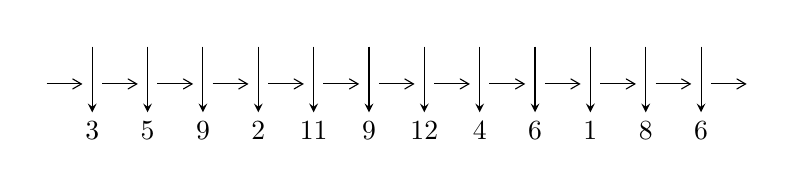
\begin{tikzpicture}[x=20pt, y=17pt]
	% nodes
	\node (C0) at (0, 0) {};
	\node (C1) at (1, 0) {};
	\node (C1U) at (1, +1) {};
	\node (C1D) at (1, -1) {3};

	\node (C2) at (2, 0) {};
	\node (C2U) at (2, +1) {};
	\node (C2D) at (2, -1) {5};

	\node (C3) at (3, 0) {};
	\node (C3U) at (3, +1) {};
	\node (C3D) at (3, -1) {9};

	\node (C4) at (4, 0) {};
	\node (C4U) at (4, +1) {};
	\node (C4D) at (4, -1) {2};

	\node (C5) at (5, 0) {};
	\node (C5U) at (5, +1) {};
	\node (C5D) at (5, -1) {11};

	\node (C6) at (6, 0) {};
	\node (C6U) at (6, +1) {};
	\node (C6D) at (6, -1) {9};

	\node (C7) at (7, 0) {};
	\node (C7U) at (7, +1) {};
	\node (C7D) at (7, -1) {12};

	\node (C8) at (8, 0) {};
	\node (C8U) at (8, +1) {};
	\node (C8D) at (8, -1) {4};

	\node (C9) at (9, 0) {};
	\node (C9U) at (9, +1) {};
	\node (C9D) at (9, -1) {6};

	\node (C10) at (10, 0) {};
	\node (C10U) at (10, +1) {};
	\node (C10D) at (10, -1) {1};

	\node (C11) at (11, 0) {};
	\node (C11U) at (11, +1) {};
	\node (C11D) at (11, -1) {8};

	\node (C12) at (12, 0) {};
	\node (C12U) at (12, +1) {};
	\node (C12D) at (12, -1) {6};
	\node (C13) at (13, 0) {};

	% arrows
	\draw[->,>={angle 60}]
	(C0) edge (C1) (C1) edge (C2) (C2) edge (C3) (C3) edge (C4) (C4) edge (C5) (C5) edge (C6) (C6) edge (C7) (C7) edge (C8) (C8) edge (C9) (C9) edge (C10) (C10) edge (C11) (C11) edge (C12) (C12) edge (C13) ;	\draw[->,>=stealth]
	(C1U) edge (C1D) (C2U) edge (C2D) (C3U) edge (C3D) (C4U) edge (C4D) (C5U) edge (C5D) (C6U) edge (C6D) (C7U) edge (C7D) (C8U) edge (C8D) (C9U) edge (C9D) (C10U) edge (C10D) (C11U) edge (C11D) (C12U) edge (C12D) ;
	\end{tikzpicture} \\
\hhline{~~} \\& 
\textbf{Solving Sequence} \\ \cline{2-2} 
 &
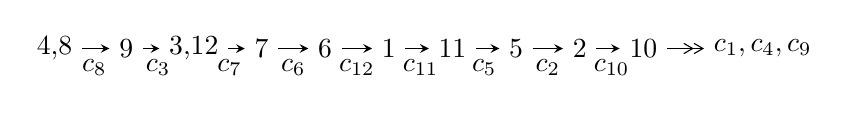
\begin{tikzpicture}[x=23pt, y=7pt]
	% node
	\node (A0) at (-1/8, 0) {4,8};
	\node (A1) at (1, 0) {9};
	\node (A2) at (33/16, 0) {3,12};
	\node (A3) at (25/8, 0) {7};
	\node (A4) at (33/8, 0) {6};
	\node (A5) at (41/8, 0) {1};
	\node (A6) at (49/8, 0) {11};
	\node (A7) at (57/8, 0) {5};
	\node (A8) at (65/8, 0) {2};
	\node (A9) at (73/8, 0) {10};
	\node (C1) at (1/2, -1) {$c_{8}$};
	\node (C2) at (3/2, -1) {$c_{3}$};
	\node (C3) at (21/8, -1) {$c_{7}$};
	\node (C4) at (29/8, -1) {$c_{6}$};
	\node (C5) at (37/8, -1) {$c_{12}$};
	\node (C6) at (45/8, -1) {$c_{11}$};
	\node (C7) at (53/8, -1) {$c_{5}$};
	\node (C8) at (61/8, -1) {$c_{2}$};
	\node (C9) at (69/8, -1) {$c_{10}$};
	\node (A10) at (11, 0) {$c_{1},c_{4},c_{9}$};

	% edge
	\draw[->,>=stealth]	
	(A0) edge (A1) (A1) edge (A2) (A2) edge (A3) (A3) edge (A4) (A4) edge (A5) (A5) edge (A6) (A6) edge (A7) (A7) edge (A8) (A8) edge (A9) ;
	\draw[->>,>={angle 60}]	
	(A9) edge (A10);
\end{tikzpicture} \\ 

\end{tabular} \\

\footnotetext{
The image of knot diagram is generated by the software ``\textbf{Draw programme}" developed by Andrew Bartholomew(\url{http://www.layer8.co.uk/maths/draw/index.htm\#Running-draw}), where we modified some parts for our purpose(\url{https://github.com/CATsTAILs/LinksPainter}).
}\phantom \\ \newline 
\centering \textbf{Ideals for irreducible components\footnotemark of $X_{\text{par}}$} 
 
\begin{align*}
I^u_{1}&=\langle 
8.06424\times10^{33} u^{29}-3.08706\times10^{34} u^{28}+\cdots+2.02678\times10^{35} b+8.88012\times10^{34},\\
\phantom{I^u_{1}}&\phantom{= \langle  }-1.10182\times10^{35} u^{29}+5.35345\times10^{35} u^{28}+\cdots+2.02678\times10^{36} a-5.52972\times10^{36},\\
\phantom{I^u_{1}}&\phantom{= \langle  }u^{30}-5 u^{29}+\cdots+208 u-64\rangle \\
I^u_{2}&=\langle 
-50322 u^{16}+60651 u^{15}+\cdots+148714 b+159141,\\
\phantom{I^u_{2}}&\phantom{= \langle  }-2740465 u^{16}+777157 u^{15}+\cdots+297428 a+8444609,\\
\phantom{I^u_{2}}&\phantom{= \langle  }u^{17}+3 u^{15}-2 u^{14}+5 u^{13}-9 u^{12}+2 u^{11}-20 u^{10}-2 u^9-25 u^8+u^7-17 u^6+6 u^5+3 u^3+2 u^2-3 u-1\rangle \\
I^u_{3}&=\langle 
-158244 u^8 a^3-40800 u^8 a^2+\cdots+813522 a-91963,\;2 u^8 a^3- u^8 a^2+\cdots+94 a+520,\\
\phantom{I^u_{3}}&\phantom{= \langle  }u^9+u^8+2 u^7+u^6+3 u^5+u^4+2 u^3+u-1\rangle \\
\\
I^v_{1}&=\langle 
a,\;b+2 v+2,\;4 v^2+6 v+1\rangle \\
\end{align*}
\raggedright * 4 irreducible components of $\dim_{\mathbb{C}}=0$, with total 85 representations.\\
\footnotetext{All coefficients of polynomials are rational numbers. But the coefficients are sometimes approximated in decimal forms when there is not enough margin.}
\newpage
\renewcommand{\arraystretch}{1}
\centering \section*{I. $I^u_{1}= \langle 8.06\times10^{33} u^{29}-3.09\times10^{34} u^{28}+\cdots+2.03\times10^{35} b+8.88\times10^{34},\;-1.10\times10^{35} u^{29}+5.35\times10^{35} u^{28}+\cdots+2.03\times10^{36} a-5.53\times10^{36},\;u^{30}-5 u^{29}+\cdots+208 u-64 \rangle$}
\flushleft \textbf{(i) Arc colorings}\\
\begin{tabular}{m{7pt} m{180pt} m{7pt} m{180pt} }
\flushright $a_{4}=$&$\begin{pmatrix}0\\u\end{pmatrix}$ \\
\flushright $a_{8}=$&$\begin{pmatrix}1\\0\end{pmatrix}$ \\
\flushright $a_{9}=$&$\begin{pmatrix}1\\u^2\end{pmatrix}$ \\
\flushright $a_{3}=$&$\begin{pmatrix}u\\u^3+u\end{pmatrix}$ \\
\flushright $a_{12}=$&$\begin{pmatrix}0.0543630 u^{29}-0.264136 u^{28}+\cdots-10.6974 u+2.72833\\-0.0397885 u^{29}+0.152314 u^{28}+\cdots-0.205764 u-0.438140\end{pmatrix}$ \\
\flushright $a_{7}=$&$\begin{pmatrix}0.0394700 u^{29}-0.200918 u^{28}+\cdots-9.53676 u+4.27030\\-0.0378177 u^{29}+0.199367 u^{28}+\cdots+10.9483 u-5.71363\end{pmatrix}$ \\
\flushright $a_{6}=$&$\begin{pmatrix}0.0249093 u^{29}-0.112539 u^{28}+\cdots-1.85669 u-1.21498\\-0.0341130 u^{29}+0.167188 u^{28}+\cdots+6.77674 u-4.71681\end{pmatrix}$ \\
\flushright $a_{1}=$&$\begin{pmatrix}0.0984923 u^{29}-0.480645 u^{28}+\cdots-18.1702 u+6.77214\\0.0129199 u^{29}-0.117465 u^{28}+\cdots-13.8793 u+11.1867\end{pmatrix}$ \\
\flushright $a_{11}=$&$\begin{pmatrix}0.0145745 u^{29}-0.111822 u^{28}+\cdots-10.9032 u+2.29019\\-0.0397885 u^{29}+0.152314 u^{28}+\cdots-0.205764 u-0.438140\end{pmatrix}$ \\
\flushright $a_{5}=$&$\begin{pmatrix}0.0265616 u^{29}-0.114090 u^{28}+\cdots-0.445179 u-3.65831\\-0.0719307 u^{29}+0.366555 u^{28}+\cdots+17.7250 u-10.4304\end{pmatrix}$ \\
\flushright $a_{2}=$&$\begin{pmatrix}-0.0766915 u^{29}+0.396957 u^{28}+\cdots+20.3635 u-7.97007\\-0.00269807 u^{29}+0.0505818 u^{28}+\cdots+12.2023 u-10.7644\end{pmatrix}$ \\
\flushright $a_{10}=$&$\begin{pmatrix}0.0441293 u^{29}-0.216509 u^{28}+\cdots-7.47278 u+5.04380\\0.0527084 u^{29}-0.269779 u^{28}+\cdots-13.6736 u+11.6248\end{pmatrix}$\\&\end{tabular}
\flushleft \textbf{(ii) Obstruction class $= -1$}\\~\\
\flushleft \textbf{(iii) Cusp Shapes $= -0.171902 u^{29}+0.740462 u^{28}+\cdots+32.2278 u-42.5665$}\\~\\
\newpage\renewcommand{\arraystretch}{1}
\flushleft \textbf{(iv) u-Polynomials at the component}\newline \\
\begin{tabular}{m{50pt}|m{274pt}}
Crossings & \hspace{64pt}u-Polynomials at each crossing \\
\hline $$\begin{aligned}c_{1}\end{aligned}$$&$\begin{aligned}
&u^{30}+17 u^{29}+\cdots+6768 u+256
\end{aligned}$\\
\hline $$\begin{aligned}c_{2},c_{4}\end{aligned}$$&$\begin{aligned}
&u^{30}-3 u^{29}+\cdots-44 u-16
\end{aligned}$\\
\hline $$\begin{aligned}c_{3},c_{8}\end{aligned}$$&$\begin{aligned}
&u^{30}-5 u^{29}+\cdots+208 u-64
\end{aligned}$\\
\hline $$\begin{aligned}c_{5},c_{7},c_{11}\end{aligned}$$&$\begin{aligned}
&u^{30}- u^{29}+\cdots+2 u^2-1
\end{aligned}$\\
\hline $$\begin{aligned}c_{6},c_{9},c_{12}\end{aligned}$$&$\begin{aligned}
&u^{30}-30 u^{28}+\cdots- u+1
\end{aligned}$\\
\hline $$\begin{aligned}c_{10}\end{aligned}$$&$\begin{aligned}
&u^{30}-19 u^{29}+\cdots+2048 u-512
\end{aligned}$\\
\hline
\end{tabular}\\~\\
\newpage\renewcommand{\arraystretch}{1}
\flushleft \textbf{(v) Riley Polynomials at the component}\newline \\
\begin{tabular}{m{50pt}|m{274pt}}
Crossings & \hspace{64pt}Riley Polynomials at each crossing \\
\hline $$\begin{aligned}c_{1}\end{aligned}$$&$\begin{aligned}
&y^{30}-5 y^{29}+\cdots-31895296 y+65536
\end{aligned}$\\
\hline $$\begin{aligned}c_{2},c_{4}\end{aligned}$$&$\begin{aligned}
&y^{30}-17 y^{29}+\cdots-6768 y+256
\end{aligned}$\\
\hline $$\begin{aligned}c_{3},c_{8}\end{aligned}$$&$\begin{aligned}
&y^{30}+9 y^{29}+\cdots-21248 y+4096
\end{aligned}$\\
\hline $$\begin{aligned}c_{5},c_{7},c_{11}\end{aligned}$$&$\begin{aligned}
&y^{30}+y^{29}+\cdots-4 y+1
\end{aligned}$\\
\hline $$\begin{aligned}c_{6},c_{9},c_{12}\end{aligned}$$&$\begin{aligned}
&y^{30}-60 y^{29}+\cdots-63 y+1
\end{aligned}$\\
\hline $$\begin{aligned}c_{10}\end{aligned}$$&$\begin{aligned}
&y^{30}-23 y^{29}+\cdots-3145728 y+262144
\end{aligned}$\\
\hline
\end{tabular}\\~\\
\newpage\flushleft \textbf{(vi) Complex Volumes and Cusp Shapes}
$$\begin{array}{c|c|c}  
\text{Solutions to }I^u_{1}& \I (\text{vol} + \sqrt{-1}CS) & \text{Cusp shape}\\
 \hline 
\begin{aligned}
u &= -0.920671 + 0.215050 I \\
a &= \phantom{-}0.474770 + 0.236439 I \\
b &= \phantom{-}0.185709 - 0.495074 I\end{aligned}
 & -0.678358 - 0.594987 I & -11.14828 - 1.26949 I \\ \hline\begin{aligned}
u &= -0.920671 - 0.215050 I \\
a &= \phantom{-}0.474770 - 0.236439 I \\
b &= \phantom{-}0.185709 + 0.495074 I\end{aligned}
 & -0.678358 + 0.594987 I & -11.14828 + 1.26949 I \\ \hline\begin{aligned}
u &= \phantom{-}0.997695 + 0.376702 I \\
a &= \phantom{-}0.437212 + 0.126971 I \\
b &= \phantom{-}0.612963 - 0.562757 I\end{aligned}
 & -1.30376 + 3.43482 I & -13.9978 - 7.1058 I \\ \hline\begin{aligned}
u &= \phantom{-}0.997695 - 0.376702 I \\
a &= \phantom{-}0.437212 - 0.126971 I \\
b &= \phantom{-}0.612963 + 0.562757 I\end{aligned}
 & -1.30376 - 3.43482 I & -13.9978 + 7.1058 I \\ \hline\begin{aligned}
u &= \phantom{-}0.316298 + 0.849109 I \\
a &= \phantom{-}0.425852 + 0.030660 I \\
b &= \phantom{-}0.918017 - 0.164528 I\end{aligned}
 & -2.07471 - 1.64401 I & -10.99207 + 2.69705 I \\ \hline\begin{aligned}
u &= \phantom{-}0.316298 - 0.849109 I \\
a &= \phantom{-}0.425852 - 0.030660 I \\
b &= \phantom{-}0.918017 + 0.164528 I\end{aligned}
 & -2.07471 + 1.64401 I & -10.99207 - 2.69705 I \\ \hline\begin{aligned}
u &= \phantom{-}0.250072 + 0.795467 I \\
a &= \phantom{-}0.08474 + 1.97666 I \\
b &= -0.528572 - 0.417784 I\end{aligned}
 & -2.30189 - 1.11843 I & -12.20818 + 6.54898 I \\ \hline\begin{aligned}
u &= \phantom{-}0.250072 - 0.795467 I \\
a &= \phantom{-}0.08474 - 1.97666 I \\
b &= -0.528572 + 0.417784 I\end{aligned}
 & -2.30189 + 1.11843 I & -12.20818 - 6.54898 I \\ \hline\begin{aligned}
u &= -0.439076 + 1.238770 I \\
a &= -0.341907 - 1.274950 I \\
b &= -0.664768 + 0.726793 I\end{aligned}
 & \phantom{-}3.50589 + 3.81678 I & -10.18184 - 5.51966 I \\ \hline\begin{aligned}
u &= -0.439076 - 1.238770 I \\
a &= -0.341907 + 1.274950 I \\
b &= -0.664768 - 0.726793 I\end{aligned}
 & \phantom{-}3.50589 - 3.81678 I & -10.18184 + 5.51966 I\\
 \hline 
 \end{array}$$\newpage$$\begin{array}{c|c|c}  
\text{Solutions to }I^u_{1}& \I (\text{vol} + \sqrt{-1}CS) & \text{Cusp shape}\\
 \hline 
\begin{aligned}
u &= \phantom{-}0.672305 + 0.131504 I \\
a &= \phantom{-}0.465097 - 0.014978 I \\
b &= -1.333120 + 0.111490 I\end{aligned}
 & -10.75090 - 0.00550 I & -26.5001 + 2.7456 I \\ \hline\begin{aligned}
u &= \phantom{-}0.672305 - 0.131504 I \\
a &= \phantom{-}0.465097 + 0.014978 I \\
b &= -1.333120 - 0.111490 I\end{aligned}
 & -10.75090 + 0.00550 I & -26.5001 - 2.7456 I \\ \hline\begin{aligned}
u &= \phantom{-}0.673336 + 1.153840 I \\
a &= -0.01039 - 1.60109 I \\
b &= \phantom{-}0.938705 + 0.985912 I\end{aligned}
 & -8.26944 - 5.68185 I & -13.8804 + 4.5637 I \\ \hline\begin{aligned}
u &= \phantom{-}0.673336 - 1.153840 I \\
a &= -0.01039 + 1.60109 I \\
b &= \phantom{-}0.938705 - 0.985912 I\end{aligned}
 & -8.26944 + 5.68185 I & -13.8804 - 4.5637 I \\ \hline\begin{aligned}
u &= -1.195980 + 0.596147 I \\
a &= \phantom{-}0.433700 + 0.140568 I \\
b &= -0.804031 - 0.882885 I\end{aligned}
 & -5.01474 - 3.34334 I & -11.59669 + 2.94079 I \\ \hline\begin{aligned}
u &= -1.195980 - 0.596147 I \\
a &= \phantom{-}0.433700 - 0.140568 I \\
b &= -0.804031 + 0.882885 I\end{aligned}
 & -5.01474 + 3.34334 I & -11.59669 - 2.94079 I \\ \hline\begin{aligned}
u &= \phantom{-}1.165670 + 0.733627 I \\
a &= \phantom{-}0.464934 - 0.150862 I \\
b &= -0.96952 + 1.09583 I\end{aligned}
 & -7.65940 + 8.88821 I & -13.8511 - 5.5347 I \\ \hline\begin{aligned}
u &= \phantom{-}1.165670 - 0.733627 I \\
a &= \phantom{-}0.464934 + 0.150862 I \\
b &= -0.96952 - 1.09583 I\end{aligned}
 & -7.65940 - 8.88821 I & -13.8511 + 5.5347 I \\ \hline\begin{aligned}
u &= \phantom{-}0.221400 + 1.363400 I \\
a &= \phantom{-}0.015740 - 1.022660 I \\
b &= -0.132717 + 0.871865 I\end{aligned}
 & \phantom{-}4.53000 - 0.32057 I & -7.71560 - 1.10595 I \\ \hline\begin{aligned}
u &= \phantom{-}0.221400 - 1.363400 I \\
a &= \phantom{-}0.015740 + 1.022660 I \\
b &= -0.132717 - 0.871865 I\end{aligned}
 & \phantom{-}4.53000 + 0.32057 I & -7.71560 + 1.10595 I\\
 \hline 
 \end{array}$$\newpage$$\begin{array}{c|c|c}  
\text{Solutions to }I^u_{1}& \I (\text{vol} + \sqrt{-1}CS) & \text{Cusp shape}\\
 \hline 
\begin{aligned}
u &= \phantom{-}0.647790 + 1.222820 I \\
a &= -0.535702 + 1.224120 I \\
b &= -0.802016 - 0.702401 I\end{aligned}
 & \phantom{-}1.35480 - 9.44263 I & -13.2001 + 10.5014 I \\ \hline\begin{aligned}
u &= \phantom{-}0.647790 - 1.222820 I \\
a &= -0.535702 - 1.224120 I \\
b &= -0.802016 + 0.702401 I\end{aligned}
 & \phantom{-}1.35480 + 9.44263 I & -13.2001 - 10.5014 I \\ \hline\begin{aligned}
u &= \phantom{-}1.40325\phantom{ +0.000000I} \\
a &= \phantom{-}0.323081\phantom{ +0.000000I} \\
b &= -0.580884\phantom{ +0.000000I}\end{aligned}
 & -10.9270\phantom{ +0.000000I} & -40.4210\phantom{ +0.000000I} \\ \hline\begin{aligned}
u &= -0.79217 + 1.21119 I \\
a &= \phantom{-}0.24417 + 1.46527 I \\
b &= \phantom{-}0.94680 - 1.23179 I\end{aligned}
 & -2.95388 + 10.39440 I & -10.10326 - 5.62687 I \\ \hline\begin{aligned}
u &= -0.79217 - 1.21119 I \\
a &= \phantom{-}0.24417 - 1.46527 I \\
b &= \phantom{-}0.94680 + 1.23179 I\end{aligned}
 & -2.95388 - 10.39440 I & -10.10326 + 5.62687 I \\ \hline\begin{aligned}
u &= \phantom{-}0.86453 + 1.17030 I \\
a &= \phantom{-}0.39716 - 1.50383 I \\
b &= \phantom{-}1.07853 + 1.31263 I\end{aligned}
 & -6.1786 - 16.1705 I & -12.9056 + 8.4851 I \\ \hline\begin{aligned}
u &= \phantom{-}0.86453 - 1.17030 I \\
a &= \phantom{-}0.39716 + 1.50383 I \\
b &= \phantom{-}1.07853 - 1.31263 I\end{aligned}
 & -6.1786 + 16.1705 I & -12.9056 - 8.4851 I \\ \hline\begin{aligned}
u &= -0.43744 + 1.41584 I \\
a &= -0.014032 + 1.010380 I \\
b &= \phantom{-}0.154110 - 0.976877 I\end{aligned}
 & \phantom{-}3.27546 + 6.39941 I & -8.60195 - 5.42628 I \\ \hline\begin{aligned}
u &= -0.43744 - 1.41584 I \\
a &= -0.014032 - 1.010380 I \\
b &= \phantom{-}0.154110 + 0.976877 I\end{aligned}
 & \phantom{-}3.27546 - 6.39941 I & -8.60195 + 5.42628 I \\ \hline\begin{aligned}
u &= -0.450762\phantom{ +0.000000I} \\
a &= \phantom{-}0.594234\phantom{ +0.000000I} \\
b &= \phantom{-}0.380692\phantom{ +0.000000I}\end{aligned}
 & -0.635586\phantom{ +0.000000I} & -15.5630\phantom{ +0.000000I}\\
 \hline 
 \end{array}$$\newpage\newpage\renewcommand{\arraystretch}{1}
\centering \section*{II. $I^u_{2}= \langle -5.03\times10^{4} u^{16}+6.07\times10^{4} u^{15}+\cdots+1.49\times10^{5} b+1.59\times10^{5},\;-2.74\times10^{6} u^{16}+7.77\times10^{5} u^{15}+\cdots+2.97\times10^{5} a+8.44\times10^{6},\;u^{17}+3 u^{15}+\cdots-3 u-1 \rangle$}
\flushleft \textbf{(i) Arc colorings}\\
\begin{tabular}{m{7pt} m{180pt} m{7pt} m{180pt} }
\flushright $a_{4}=$&$\begin{pmatrix}0\\u\end{pmatrix}$ \\
\flushright $a_{8}=$&$\begin{pmatrix}1\\0\end{pmatrix}$ \\
\flushright $a_{9}=$&$\begin{pmatrix}1\\u^2\end{pmatrix}$ \\
\flushright $a_{3}=$&$\begin{pmatrix}u\\u^3+u\end{pmatrix}$ \\
\flushright $a_{12}=$&$\begin{pmatrix}9.21388 u^{16}-2.61292 u^{15}+\cdots+9.55963 u-28.3921\\0.338381 u^{16}-0.407837 u^{15}+\cdots+0.429865 u-1.07011\end{pmatrix}$ \\
\flushright $a_{7}=$&$\begin{pmatrix}8.05673 u^{16}-2.39322 u^{15}+\cdots+5.18074 u-23.8643\\0.240774 u^{16}+0.356863 u^{15}+\cdots+0.945237 u-0.542810\end{pmatrix}$ \\
\flushright $a_{6}=$&$\begin{pmatrix}7.15244 u^{16}-2.00192 u^{15}+\cdots+5.24891 u-22.0139\\0.161686 u^{16}+0.219011 u^{15}+\cdots+1.21485 u-0.151512\end{pmatrix}$ \\
\flushright $a_{1}=$&$\begin{pmatrix}1.06597 u^{16}-0.172287 u^{15}+\cdots+1.14668 u-3.00192\\-0.00475409 u^{16}-0.200035 u^{15}+\cdots+0.818719 u+0.219011\end{pmatrix}$ \\
\flushright $a_{11}=$&$\begin{pmatrix}9.55226 u^{16}-3.02076 u^{15}+\cdots+9.98950 u-29.4622\\0.338381 u^{16}-0.407837 u^{15}+\cdots+0.429865 u-1.07011\end{pmatrix}$ \\
\flushright $a_{5}=$&$\begin{pmatrix}-1.14506 u^{16}+0.0344352 u^{15}+\cdots-0.877073 u+3.39322\\-0.0790880 u^{16}-0.137852 u^{15}+\cdots+0.269611 u+0.391298\end{pmatrix}$ \\
\flushright $a_{2}=$&$\begin{pmatrix}1.11352 u^{16}-0.409703 u^{15}+\cdots+2.18844 u-3.03636\\0.179102 u^{16}-0.186802 u^{15}+\cdots+1.19578 u-0.0528397\end{pmatrix}$ \\
\flushright $a_{10}=$&$\begin{pmatrix}8.14791 u^{16}-2.44064 u^{15}+\cdots+8.41295 u-24.3902\\0.343135 u^{16}-0.207802 u^{15}+\cdots-0.388854 u-1.28913\end{pmatrix}$\\&\end{tabular}
\flushleft \textbf{(ii) Obstruction class $= 1$}\\~\\
\flushleft \textbf{(iii) Cusp Shapes $= \frac{6794471}{297428} u^{16}-\frac{1681861}{297428} u^{15}+\cdots+\frac{571348}{74357} u-\frac{25623465}{297428}$}\\~\\
\newpage\renewcommand{\arraystretch}{1}
\flushleft \textbf{(iv) u-Polynomials at the component}\newline \\
\begin{tabular}{m{50pt}|m{274pt}}
Crossings & \hspace{64pt}u-Polynomials at each crossing \\
\hline $$\begin{aligned}c_{1}\end{aligned}$$&$\begin{aligned}
&u^{17}-10 u^{16}+\cdots+17 u-1
\end{aligned}$\\
\hline $$\begin{aligned}c_{2}\end{aligned}$$&$\begin{aligned}
&u^{17}+4 u^{16}+\cdots- u+1
\end{aligned}$\\
\hline $$\begin{aligned}c_{3}\end{aligned}$$&$\begin{aligned}
&u^{17}+3 u^{15}+\cdots-3 u+1
\end{aligned}$\\
\hline $$\begin{aligned}c_{4}\end{aligned}$$&$\begin{aligned}
&u^{17}-4 u^{16}+\cdots- u-1
\end{aligned}$\\
\hline $$\begin{aligned}c_{5},c_{11}\end{aligned}$$&$\begin{aligned}
&u^{17}+6 u^{15}+\cdots-3 u-1
\end{aligned}$\\
\hline $$\begin{aligned}c_{6},c_{12}\end{aligned}$$&$\begin{aligned}
&u^{17}-3 u^{16}+\cdots+6 u^2+1
\end{aligned}$\\
\hline $$\begin{aligned}c_{7}\end{aligned}$$&$\begin{aligned}
&u^{17}+6 u^{15}+\cdots-3 u+1
\end{aligned}$\\
\hline $$\begin{aligned}c_{8}\end{aligned}$$&$\begin{aligned}
&u^{17}+3 u^{15}+\cdots-3 u-1
\end{aligned}$\\
\hline $$\begin{aligned}c_{9}\end{aligned}$$&$\begin{aligned}
&u^{17}+3 u^{16}+\cdots-6 u^2-1
\end{aligned}$\\
\hline $$\begin{aligned}c_{10}\end{aligned}$$&$\begin{aligned}
&u^{17}-5 u^{16}+\cdots+5 u-1
\end{aligned}$\\
\hline
\end{tabular}\\~\\
\newpage\renewcommand{\arraystretch}{1}
\flushleft \textbf{(v) Riley Polynomials at the component}\newline \\
\begin{tabular}{m{50pt}|m{274pt}}
Crossings & \hspace{64pt}Riley Polynomials at each crossing \\
\hline $$\begin{aligned}c_{1}\end{aligned}$$&$\begin{aligned}
&y^{17}-2 y^{16}+\cdots+157 y-1
\end{aligned}$\\
\hline $$\begin{aligned}c_{2},c_{4}\end{aligned}$$&$\begin{aligned}
&y^{17}-10 y^{16}+\cdots+17 y-1
\end{aligned}$\\
\hline $$\begin{aligned}c_{3},c_{8}\end{aligned}$$&$\begin{aligned}
&y^{17}+6 y^{16}+\cdots+13 y-1
\end{aligned}$\\
\hline $$\begin{aligned}c_{5},c_{7},c_{11}\end{aligned}$$&$\begin{aligned}
&y^{17}+12 y^{16}+\cdots+5 y-1
\end{aligned}$\\
\hline $$\begin{aligned}c_{6},c_{9},c_{12}\end{aligned}$$&$\begin{aligned}
&y^{17}-5 y^{16}+\cdots-12 y-1
\end{aligned}$\\
\hline $$\begin{aligned}c_{10}\end{aligned}$$&$\begin{aligned}
&y^{17}-17 y^{16}+\cdots+11 y-1
\end{aligned}$\\
\hline
\end{tabular}\\~\\
\newpage\flushleft \textbf{(vi) Complex Volumes and Cusp Shapes}
$$\begin{array}{c|c|c}  
\text{Solutions to }I^u_{2}& \I (\text{vol} + \sqrt{-1}CS) & \text{Cusp shape}\\
 \hline 
\begin{aligned}
u &= -0.222868 + 0.957169 I \\
a &= \phantom{-}0.937935 - 0.366003 I \\
b &= \phantom{-}0.975905 + 0.087227 I\end{aligned}
 & -3.24280 + 2.04185 I & -17.4447 - 3.6628 I \\ \hline\begin{aligned}
u &= -0.222868 - 0.957169 I \\
a &= \phantom{-}0.937935 + 0.366003 I \\
b &= \phantom{-}0.975905 - 0.087227 I\end{aligned}
 & -3.24280 - 2.04185 I & -17.4447 + 3.6628 I \\ \hline\begin{aligned}
u &= -0.143073 + 1.125680 I \\
a &= -0.06490 + 1.65937 I \\
b &= -0.240226 - 1.383230 I\end{aligned}
 & \phantom{-}6.60440 - 0.23148 I & -4.66739 - 0.18271 I \\ \hline\begin{aligned}
u &= -0.143073 - 1.125680 I \\
a &= -0.06490 - 1.65937 I \\
b &= -0.240226 + 1.383230 I\end{aligned}
 & \phantom{-}6.60440 + 0.23148 I & -4.66739 + 0.18271 I \\ \hline\begin{aligned}
u &= -0.934717 + 0.786177 I \\
a &= -0.460802 - 0.068107 I \\
b &= \phantom{-}0.102794 + 0.830593 I\end{aligned}
 & \phantom{-}0.49138 - 1.47201 I & -4.39198 + 2.32537 I \\ \hline\begin{aligned}
u &= -0.934717 - 0.786177 I \\
a &= -0.460802 + 0.068107 I \\
b &= \phantom{-}0.102794 - 0.830593 I\end{aligned}
 & \phantom{-}0.49138 + 1.47201 I & -4.39198 - 2.32537 I \\ \hline\begin{aligned}
u &= \phantom{-}0.463922 + 1.145870 I \\
a &= \phantom{-}0.43983 - 1.42671 I \\
b &= -0.17875 + 1.49824 I\end{aligned}
 & \phantom{-}5.30175 - 4.82160 I & -8.88387 + 5.04151 I \\ \hline\begin{aligned}
u &= \phantom{-}0.463922 - 1.145870 I \\
a &= \phantom{-}0.43983 + 1.42671 I \\
b &= -0.17875 - 1.49824 I\end{aligned}
 & \phantom{-}5.30175 + 4.82160 I & -8.88387 - 5.04151 I \\ \hline\begin{aligned}
u &= \phantom{-}0.622575 + 1.114960 I \\
a &= -0.632046 + 0.809570 I \\
b &= -0.340268 - 0.934275 I\end{aligned}
 & \phantom{-}4.76952 - 2.66666 I & -3.51429 + 3.01636 I \\ \hline\begin{aligned}
u &= \phantom{-}0.622575 - 1.114960 I \\
a &= -0.632046 - 0.809570 I \\
b &= -0.340268 + 0.934275 I\end{aligned}
 & \phantom{-}4.76952 + 2.66666 I & -3.51429 - 3.01636 I\\
 \hline 
 \end{array}$$\newpage$$\begin{array}{c|c|c}  
\text{Solutions to }I^u_{2}& \I (\text{vol} + \sqrt{-1}CS) & \text{Cusp shape}\\
 \hline 
\begin{aligned}
u &= \phantom{-}0.621513 + 0.226133 I \\
a &= \phantom{-}3.17814 + 0.77491 I \\
b &= \phantom{-}0.068320 + 1.335540 I\end{aligned}
 & \phantom{-}2.59448 + 0.58189 I & -16.1225 - 5.9646 I \\ \hline\begin{aligned}
u &= \phantom{-}0.621513 - 0.226133 I \\
a &= \phantom{-}3.17814 - 0.77491 I \\
b &= \phantom{-}0.068320 - 1.335540 I\end{aligned}
 & \phantom{-}2.59448 - 0.58189 I & -16.1225 + 5.9646 I \\ \hline\begin{aligned}
u &= -0.76282 + 1.20700 I \\
a &= -0.450462 - 0.871861 I \\
b &= -0.529361 + 0.773457 I\end{aligned}
 & \phantom{-}1.99341 + 8.23287 I & -9.38259 - 6.87786 I \\ \hline\begin{aligned}
u &= -0.76282 - 1.20700 I \\
a &= -0.450462 + 0.871861 I \\
b &= -0.529361 - 0.773457 I\end{aligned}
 & \phantom{-}1.99341 - 8.23287 I & -9.38259 + 6.87786 I \\ \hline\begin{aligned}
u &= -0.509710\phantom{ +0.000000I} \\
a &= -3.08687\phantom{ +0.000000I} \\
b &= \phantom{-}0.727999\phantom{ +0.000000I}\end{aligned}
 & -4.29378\phantom{ +0.000000I} & -7.87230\phantom{ +0.000000I} \\ \hline\begin{aligned}
u &= \phantom{-}1.53136\phantom{ +0.000000I} \\
a &= -0.327837\phantom{ +0.000000I} \\
b &= \phantom{-}0.362879\phantom{ +0.000000I}\end{aligned}
 & -10.7956\phantom{ +0.000000I} & \phantom{-}20.7800\phantom{ +0.000000I} \\ \hline\begin{aligned}
u &= -0.310720\phantom{ +0.000000I} \\
a &= -25.4807\phantom{ +0.000000I} \\
b &= -0.807701\phantom{ +0.000000I}\end{aligned}
 & -5.48556\phantom{ +0.000000I} & -72.0930\phantom{ +0.000000I}\\
 \hline 
 \end{array}$$\newpage\newpage\renewcommand{\arraystretch}{1}
\centering \section*{III. $I^u_{3}= \langle -1.58\times10^{5} a^{3} u^{8}-4.08\times10^{4} a^{2} u^{8}+\cdots+8.14\times10^{5} a-9.20\times10^{4},\;2 u^8 a^3- u^8 a^2+\cdots+94 a+520,\;u^9+u^8+2 u^7+u^6+3 u^5+u^4+2 u^3+u-1 \rangle$}
\flushleft \textbf{(i) Arc colorings}\\
\begin{tabular}{m{7pt} m{180pt} m{7pt} m{180pt} }
\flushright $a_{4}=$&$\begin{pmatrix}0\\u\end{pmatrix}$ \\
\flushright $a_{8}=$&$\begin{pmatrix}1\\0\end{pmatrix}$ \\
\flushright $a_{9}=$&$\begin{pmatrix}1\\u^2\end{pmatrix}$ \\
\flushright $a_{3}=$&$\begin{pmatrix}u\\u^3+u\end{pmatrix}$ \\
\flushright $a_{12}=$&$\begin{pmatrix}a\\0.250587 a^{3} u^{8}+0.0646088 a^{2} u^{8}+\cdots-1.28825 a+0.145628\end{pmatrix}$ \\
\flushright $a_{7}=$&$\begin{pmatrix}0.0695431 a^{3} u^{8}-0.0718551 a^{2} u^{8}+\cdots-0.741380 a+2.26000\\-0.0275854 a^{3} u^{8}+0.352029 a^{2} u^{8}+\cdots+1.67727 a+0.105629\end{pmatrix}$ \\
\flushright $a_{6}=$&$\begin{pmatrix}-0.0695431 a^{3} u^{8}+0.0718551 a^{2} u^{8}+\cdots+0.741380 a+1.74000\\-0.250587 a^{3} u^{8}-0.0646088 a^{2} u^{8}+\cdots+1.28825 a+0.854372\end{pmatrix}$ \\
\flushright $a_{1}=$&$\begin{pmatrix}- u^2-1\\- u^2\end{pmatrix}$ \\
\flushright $a_{11}=$&$\begin{pmatrix}0.250587 a^{3} u^{8}+0.0646088 a^{2} u^{8}+\cdots-0.288252 a+0.145628\\0.250587 a^{3} u^{8}+0.0646088 a^{2} u^{8}+\cdots-1.28825 a+0.145628\end{pmatrix}$ \\
\flushright $a_{5}=$&$\begin{pmatrix}- u^4- u^2-1\\- u^4\end{pmatrix}$ \\
\flushright $a_{2}=$&$\begin{pmatrix}u^6+u^4+2 u^2+1\\u^8+2 u^6+2 u^4+2 u^2\end{pmatrix}$ \\
\flushright $a_{10}=$&$\begin{pmatrix}0.324754 a^{3} u^{8}+0.342471 a^{2} u^{8}+\cdots-0.326854 a+0.340849\\0.0741671 a^{3} u^{8}+0.277862 a^{2} u^{8}+\cdots-0.0386022 a+0.195221\end{pmatrix}$\\&\end{tabular}
\flushleft \textbf{(ii) Obstruction class $= -1$}\\~\\
\flushleft \textbf{(iii) Cusp Shapes $= -4 u^7-4 u^6-4 u^5-4 u^4-8 u^3-4 u^2-14$}\\~\\
\newpage\renewcommand{\arraystretch}{1}
\flushleft \textbf{(iv) u-Polynomials at the component}\newline \\
\begin{tabular}{m{50pt}|m{274pt}}
Crossings & \hspace{64pt}u-Polynomials at each crossing \\
\hline $$\begin{aligned}c_{1}\end{aligned}$$&$\begin{aligned}
&(u^9+5 u^8+12 u^7+15 u^6+9 u^5- u^4-4 u^3-2 u^2+u+1)^4
\end{aligned}$\\
\hline $$\begin{aligned}c_{2},c_{4}\end{aligned}$$&$\begin{aligned}
&(u^9- u^8-2 u^7+3 u^6+u^5-3 u^4+2 u^3- u+1)^4
\end{aligned}$\\
\hline $$\begin{aligned}c_{3},c_{8}\end{aligned}$$&$\begin{aligned}
&(u^9+u^8+2 u^7+u^6+3 u^5+u^4+2 u^3+u-1)^4
\end{aligned}$\\
\hline $$\begin{aligned}c_{5},c_{7},c_{11}\end{aligned}$$&$\begin{aligned}
&u^{36}+3 u^{35}+\cdots-136 u-31
\end{aligned}$\\
\hline $$\begin{aligned}c_{6},c_{9},c_{12}\end{aligned}$$&$\begin{aligned}
&u^{36}-3 u^{35}+\cdots+18264 u-3559
\end{aligned}$\\
\hline $$\begin{aligned}c_{10}\end{aligned}$$&$\begin{aligned}
&(u^2+u-1)^{18}
\end{aligned}$\\
\hline
\end{tabular}\\~\\
\newpage\renewcommand{\arraystretch}{1}
\flushleft \textbf{(v) Riley Polynomials at the component}\newline \\
\begin{tabular}{m{50pt}|m{274pt}}
Crossings & \hspace{64pt}Riley Polynomials at each crossing \\
\hline $$\begin{aligned}c_{1}\end{aligned}$$&$\begin{aligned}
&(y^9- y^8+12 y^7-7 y^6+37 y^5+y^4-10 y^2+5 y-1)^4
\end{aligned}$\\
\hline $$\begin{aligned}c_{2},c_{4}\end{aligned}$$&$\begin{aligned}
&(y^9-5 y^8+12 y^7-15 y^6+9 y^5+y^4-4 y^3+2 y^2+y-1)^4
\end{aligned}$\\
\hline $$\begin{aligned}c_{3},c_{8}\end{aligned}$$&$\begin{aligned}
&(y^9+3 y^8+8 y^7+13 y^6+17 y^5+17 y^4+12 y^3+6 y^2+y-1)^4
\end{aligned}$\\
\hline $$\begin{aligned}c_{5},c_{7},c_{11}\end{aligned}$$&$\begin{aligned}
&y^{36}+11 y^{35}+\cdots+16224 y+961
\end{aligned}$\\
\hline $$\begin{aligned}c_{6},c_{9},c_{12}\end{aligned}$$&$\begin{aligned}
&y^{36}-25 y^{35}+\cdots+545224 y+12666481
\end{aligned}$\\
\hline $$\begin{aligned}c_{10}\end{aligned}$$&$\begin{aligned}
&(y^2-3 y+1)^{18}
\end{aligned}$\\
\hline
\end{tabular}\\~\\
\newpage\flushleft \textbf{(vi) Complex Volumes and Cusp Shapes}
$$\begin{array}{c|c|c}  
\text{Solutions to }I^u_{3}& \I (\text{vol} + \sqrt{-1}CS) & \text{Cusp shape}\\
 \hline 
\begin{aligned}
u &= \phantom{-}0.140343 + 0.966856 I \\
a &= -0.61869 + 1.39310 I \\
b &= -0.42993 - 1.44275 I\end{aligned}
 & \phantom{-}5.73128 - 2.09337 I & -7.48501 + 4.16283 I \\ \hline\begin{aligned}
u &= \phantom{-}0.140343 + 0.966856 I \\
a &= \phantom{-}1.38851 + 0.80504 I \\
b &= \phantom{-}0.128913 - 0.359883 I\end{aligned}
 & -2.16441 - 2.09337 I & -7.48501 + 4.16283 I \\ \hline\begin{aligned}
u &= \phantom{-}0.140343 + 0.966856 I \\
a &= \phantom{-}0.243842 + 0.158886 I \\
b &= \phantom{-}1.351770 - 0.079224 I\end{aligned}
 & -2.16441 - 2.09337 I & -7.48501 + 4.16283 I \\ \hline\begin{aligned}
u &= \phantom{-}0.140343 + 0.966856 I \\
a &= -0.00482 - 1.76129 I \\
b &= -0.13564 + 1.61047 I\end{aligned}
 & \phantom{-}5.73128 - 2.09337 I & -7.48501 + 4.16283 I \\ \hline\begin{aligned}
u &= \phantom{-}0.140343 - 0.966856 I \\
a &= -0.61869 - 1.39310 I \\
b &= -0.42993 + 1.44275 I\end{aligned}
 & \phantom{-}5.73128 + 2.09337 I & -7.48501 - 4.16283 I \\ \hline\begin{aligned}
u &= \phantom{-}0.140343 - 0.966856 I \\
a &= \phantom{-}1.38851 - 0.80504 I \\
b &= \phantom{-}0.128913 + 0.359883 I\end{aligned}
 & -2.16441 + 2.09337 I & -7.48501 - 4.16283 I \\ \hline\begin{aligned}
u &= \phantom{-}0.140343 - 0.966856 I \\
a &= \phantom{-}0.243842 - 0.158886 I \\
b &= \phantom{-}1.351770 + 0.079224 I\end{aligned}
 & -2.16441 + 2.09337 I & -7.48501 - 4.16283 I \\ \hline\begin{aligned}
u &= \phantom{-}0.140343 - 0.966856 I \\
a &= -0.00482 + 1.76129 I \\
b &= -0.13564 - 1.61047 I\end{aligned}
 & \phantom{-}5.73128 + 2.09337 I & -7.48501 - 4.16283 I \\ \hline\begin{aligned}
u &= \phantom{-}0.628449 + 0.875112 I \\
a &= -0.525443 + 0.462550 I \\
b &= \phantom{-}1.30414 - 0.74950 I\end{aligned}
 & -4.56478 - 2.45442 I & -10.32792 + 2.91298 I \\ \hline\begin{aligned}
u &= \phantom{-}0.628449 + 0.875112 I \\
a &= \phantom{-}0.763452 - 1.086660 I \\
b &= \phantom{-}0.294073 + 1.242760 I\end{aligned}
 & \phantom{-}3.33090 - 2.45442 I & -10.32792 + 2.91298 I\\
 \hline 
 \end{array}$$\newpage$$\begin{array}{c|c|c}  
\text{Solutions to }I^u_{3}& \I (\text{vol} + \sqrt{-1}CS) & \text{Cusp shape}\\
 \hline 
\begin{aligned}
u &= \phantom{-}0.628449 + 0.875112 I \\
a &= -0.485650 + 0.077610 I \\
b &= -0.523285 - 0.562963 I\end{aligned}
 & \phantom{-}3.33090 - 2.45442 I & -10.32792 + 2.91298 I \\ \hline\begin{aligned}
u &= \phantom{-}0.628449 + 0.875112 I \\
a &= -0.20185 + 2.17919 I \\
b &= -0.704050 - 1.030220 I\end{aligned}
 & -4.56478 - 2.45442 I & -10.32792 + 2.91298 I \\ \hline\begin{aligned}
u &= \phantom{-}0.628449 - 0.875112 I \\
a &= -0.525443 - 0.462550 I \\
b &= \phantom{-}1.30414 + 0.74950 I\end{aligned}
 & -4.56478 + 2.45442 I & -10.32792 - 2.91298 I \\ \hline\begin{aligned}
u &= \phantom{-}0.628449 - 0.875112 I \\
a &= \phantom{-}0.763452 + 1.086660 I \\
b &= \phantom{-}0.294073 - 1.242760 I\end{aligned}
 & \phantom{-}3.33090 + 2.45442 I & -10.32792 - 2.91298 I \\ \hline\begin{aligned}
u &= \phantom{-}0.628449 - 0.875112 I \\
a &= -0.485650 - 0.077610 I \\
b &= -0.523285 + 0.562963 I\end{aligned}
 & \phantom{-}3.33090 + 2.45442 I & -10.32792 - 2.91298 I \\ \hline\begin{aligned}
u &= \phantom{-}0.628449 - 0.875112 I \\
a &= -0.20185 - 2.17919 I \\
b &= -0.704050 + 1.030220 I\end{aligned}
 & -4.56478 + 2.45442 I & -10.32792 - 2.91298 I \\ \hline\begin{aligned}
u &= -0.796005 + 0.733148 I \\
a &= -0.880986 - 0.487136 I \\
b &= \phantom{-}0.964779 + 0.981447 I\end{aligned}
 & -8.31919 - 1.33617 I & -15.2841 + 0.7017 I \\ \hline\begin{aligned}
u &= -0.796005 + 0.733148 I \\
a &= \phantom{-}0.892032 + 0.347149 I \\
b &= -0.127108 - 1.007800 I\end{aligned}
 & -0.423507 - 1.336170 I & -15.2841 + 0.7017 I \\ \hline\begin{aligned}
u &= -0.796005 + 0.733148 I \\
a &= -0.187374 + 0.704738 I \\
b &= \phantom{-}0.186512 + 0.286438 I\end{aligned}
 & -0.423507 - 1.336170 I & -15.2841 + 0.7017 I \\ \hline\begin{aligned}
u &= -0.796005 + 0.733148 I \\
a &= -0.96383 - 2.26674 I \\
b &= -1.12030 + 0.90709 I\end{aligned}
 & -8.31919 - 1.33617 I & -15.2841 + 0.7017 I\\
 \hline 
 \end{array}$$\newpage$$\begin{array}{c|c|c}  
\text{Solutions to }I^u_{3}& \I (\text{vol} + \sqrt{-1}CS) & \text{Cusp shape}\\
 \hline 
\begin{aligned}
u &= -0.796005 - 0.733148 I \\
a &= -0.880986 + 0.487136 I \\
b &= \phantom{-}0.964779 - 0.981447 I\end{aligned}
 & -8.31919 + 1.33617 I & -15.2841 - 0.7017 I \\ \hline\begin{aligned}
u &= -0.796005 - 0.733148 I \\
a &= \phantom{-}0.892032 - 0.347149 I \\
b &= -0.127108 + 1.007800 I\end{aligned}
 & -0.423507 + 1.336170 I & -15.2841 - 0.7017 I \\ \hline\begin{aligned}
u &= -0.796005 - 0.733148 I \\
a &= -0.187374 - 0.704738 I \\
b &= \phantom{-}0.186512 - 0.286438 I\end{aligned}
 & -0.423507 + 1.336170 I & -15.2841 - 0.7017 I \\ \hline\begin{aligned}
u &= -0.796005 - 0.733148 I \\
a &= -0.96383 + 2.26674 I \\
b &= -1.12030 - 0.90709 I\end{aligned}
 & -8.31919 + 1.33617 I & -15.2841 - 0.7017 I \\ \hline\begin{aligned}
u &= -0.728966 + 0.986295 I \\
a &= \phantom{-}0.501545 + 1.033540 I \\
b &= \phantom{-}0.646764 - 1.177390 I\end{aligned}
 & \phantom{-}0.34972 + 7.08493 I & -13.5768 - 5.9133 I \\ \hline\begin{aligned}
u &= -0.728966 + 0.986295 I \\
a &= -0.593832 - 0.265649 I \\
b &= \phantom{-}1.49815 + 0.97115 I\end{aligned}
 & -7.54597 + 7.08493 I & -13.5768 - 5.9133 I \\ \hline\begin{aligned}
u &= -0.728966 + 0.986295 I \\
a &= -0.124651 - 0.247951 I \\
b &= -0.919556 + 0.288684 I\end{aligned}
 & \phantom{-}0.34972 + 7.08493 I & -13.5768 - 5.9133 I \\ \hline\begin{aligned}
u &= -0.728966 + 0.986295 I \\
a &= -0.39289 - 1.79104 I \\
b &= -0.78397 + 1.35550 I\end{aligned}
 & -7.54597 + 7.08493 I & -13.5768 - 5.9133 I \\ \hline\begin{aligned}
u &= -0.728966 - 0.986295 I \\
a &= \phantom{-}0.501545 - 1.033540 I \\
b &= \phantom{-}0.646764 + 1.177390 I\end{aligned}
 & \phantom{-}0.34972 - 7.08493 I & -13.5768 + 5.9133 I \\ \hline\begin{aligned}
u &= -0.728966 - 0.986295 I \\
a &= -0.593832 + 0.265649 I \\
b &= \phantom{-}1.49815 - 0.97115 I\end{aligned}
 & -7.54597 - 7.08493 I & -13.5768 + 5.9133 I\\
 \hline 
 \end{array}$$\newpage$$\begin{array}{c|c|c}  
\text{Solutions to }I^u_{3}& \I (\text{vol} + \sqrt{-1}CS) & \text{Cusp shape}\\
 \hline 
\begin{aligned}
u &= -0.728966 - 0.986295 I \\
a &= -0.124651 + 0.247951 I \\
b &= -0.919556 - 0.288684 I\end{aligned}
 & \phantom{-}0.34972 - 7.08493 I & -13.5768 + 5.9133 I \\ \hline\begin{aligned}
u &= -0.728966 - 0.986295 I \\
a &= -0.39289 + 1.79104 I \\
b &= -0.78397 - 1.35550 I\end{aligned}
 & -7.54597 - 7.08493 I & -13.5768 + 5.9133 I \\ \hline\begin{aligned}
u &= \phantom{-}0.512358\phantom{ +0.000000I} \\
a &= -4.03622\phantom{ +0.000000I} \\
b &= \phantom{-}0.558485\phantom{ +0.000000I}\end{aligned}
 & -5.14629\phantom{ +0.000000I} & -16.6520\phantom{ +0.000000I} \\ \hline\begin{aligned}
u &= \phantom{-}0.512358\phantom{ +0.000000I} \\
a &= \phantom{-}2.66334 + 4.93805 I \\
b &= \phantom{-}0.081120 + 1.296290 I\end{aligned}
 & \phantom{-}2.74940\phantom{ +0.000000I} & -16.6520\phantom{ +0.000000I} \\ \hline\begin{aligned}
u &= \phantom{-}0.512358\phantom{ +0.000000I} \\
a &= \phantom{-}2.66334 - 4.93805 I \\
b &= \phantom{-}0.081120 - 1.296290 I\end{aligned}
 & \phantom{-}2.74940\phantom{ +0.000000I} & -16.6520\phantom{ +0.000000I} \\ \hline\begin{aligned}
u &= \phantom{-}0.512358\phantom{ +0.000000I} \\
a &= -9.90920\phantom{ +0.000000I} \\
b &= -0.983236\phantom{ +0.000000I}\end{aligned}
 & -5.14629\phantom{ +0.000000I} & -16.6520\phantom{ +0.000000I}\\
 \hline 
 \end{array}$$\newpage\newpage\renewcommand{\arraystretch}{1}
\centering \section*{IV. $I^v_{1}= \langle a,\;b+2 v+2,\;4 v^2+6 v+1 \rangle$}
\flushleft \textbf{(i) Arc colorings}\\
\begin{tabular}{m{7pt} m{180pt} m{7pt} m{180pt} }
\flushright $a_{4}=$&$\begin{pmatrix}v\\0\end{pmatrix}$ \\
\flushright $a_{8}=$&$\begin{pmatrix}1\\0\end{pmatrix}$ \\
\flushright $a_{9}=$&$\begin{pmatrix}1\\0\end{pmatrix}$ \\
\flushright $a_{3}=$&$\begin{pmatrix}v\\0\end{pmatrix}$ \\
\flushright $a_{12}=$&$\begin{pmatrix}0\\-2 v-2\end{pmatrix}$ \\
\flushright $a_{7}=$&$\begin{pmatrix}1\\-2 v-3\end{pmatrix}$ \\
\flushright $a_{6}=$&$\begin{pmatrix}-2 v-2\\-2 v-3\end{pmatrix}$ \\
\flushright $a_{1}=$&$\begin{pmatrix}4 v+5\\4 v+6\end{pmatrix}$ \\
\flushright $a_{11}=$&$\begin{pmatrix}-2 v-2\\-2 v-2\end{pmatrix}$ \\
\flushright $a_{5}=$&$\begin{pmatrix}-4 v-5\\-4 v-6\end{pmatrix}$ \\
\flushright $a_{2}=$&$\begin{pmatrix}5 v+5\\4 v+6\end{pmatrix}$ \\
\flushright $a_{10}=$&$\begin{pmatrix}4 v+6\\6 v+8\end{pmatrix}$\\&\end{tabular}
\flushleft \textbf{(ii) Obstruction class $= 1$}\\~\\
\flushleft \textbf{(iii) Cusp Shapes $= \frac{45}{2} v+\frac{55}{4}$}\\~\\
\newpage\renewcommand{\arraystretch}{1}
\flushleft \textbf{(iv) u-Polynomials at the component}\newline \\
\begin{tabular}{m{50pt}|m{274pt}}
Crossings & \hspace{64pt}u-Polynomials at each crossing \\
\hline $$\begin{aligned}c_{1},c_{2}\end{aligned}$$&$\begin{aligned}
&(u-1)^2
\end{aligned}$\\
\hline $$\begin{aligned}c_{3},c_{8}\end{aligned}$$&$\begin{aligned}
&u^2
\end{aligned}$\\
\hline $$\begin{aligned}c_{4}\end{aligned}$$&$\begin{aligned}
&(u+1)^2
\end{aligned}$\\
\hline $$\begin{aligned}c_{5},c_{7},c_{10}\end{aligned}$$&$\begin{aligned}
&u^2+u-1
\end{aligned}$\\
\hline $$\begin{aligned}c_{6}\end{aligned}$$&$\begin{aligned}
&u^2-3 u+1
\end{aligned}$\\
\hline $$\begin{aligned}c_{9},c_{12}\end{aligned}$$&$\begin{aligned}
&u^2+3 u+1
\end{aligned}$\\
\hline $$\begin{aligned}c_{11}\end{aligned}$$&$\begin{aligned}
&u^2- u-1
\end{aligned}$\\
\hline
\end{tabular}\\~\\
\newpage\renewcommand{\arraystretch}{1}
\flushleft \textbf{(v) Riley Polynomials at the component}\newline \\
\begin{tabular}{m{50pt}|m{274pt}}
Crossings & \hspace{64pt}Riley Polynomials at each crossing \\
\hline $$\begin{aligned}c_{1},c_{2},c_{4}\end{aligned}$$&$\begin{aligned}
&(y-1)^2
\end{aligned}$\\
\hline $$\begin{aligned}c_{3},c_{8}\end{aligned}$$&$\begin{aligned}
&y^2
\end{aligned}$\\
\hline $$\begin{aligned}c_{5},c_{7},c_{10}\\c_{11}\end{aligned}$$&$\begin{aligned}
&y^2-3 y+1
\end{aligned}$\\
\hline $$\begin{aligned}c_{6},c_{9},c_{12}\end{aligned}$$&$\begin{aligned}
&y^2-7 y+1
\end{aligned}$\\
\hline
\end{tabular}\\~\\
\newpage\flushleft \textbf{(vi) Complex Volumes and Cusp Shapes}
$$\begin{array}{c|c|c}  
\text{Solutions to }I^v_{1}& \I (\text{vol} + \sqrt{-1}CS) & \text{Cusp shape}\\
 \hline 
\begin{aligned}
v &= -1.30902\phantom{ +0.000000I} \\
a &= \phantom{-0.000000 } 0 \\
b &= \phantom{-}0.618034\phantom{ +0.000000I}\end{aligned}
 & -2.63189\phantom{ +0.000000I} & -15.7030\phantom{ +0.000000I} \\ \hline\begin{aligned}
v &= -0.190983\phantom{ +0.000000I} \\
a &= \phantom{-0.000000 } 0 \\
b &= -1.61803\phantom{ +0.000000I}\end{aligned}
 & -10.5276\phantom{ +0.000000I} & \phantom{-}9.45290\phantom{ +0.000000I}\\
 \hline 
 \end{array}$$\newpage
\newpage\renewcommand{\arraystretch}{1}
\centering \section*{ V. u-Polynomials}
\begin{tabular}{m{50pt}|m{274pt}}
Crossings & \hspace{64pt}u-Polynomials at each crossing \\
\hline $$\begin{aligned}c_{1}\end{aligned}$$&$\begin{aligned}
&(u-1)^2(u^9+5 u^8+12 u^7+15 u^6+9 u^5- u^4-4 u^3-2 u^2+u+1)^4\\
&\cdot(u^{17}-10 u^{16}+\cdots+17 u-1)(u^{30}+17 u^{29}+\cdots+6768 u+256)
\end{aligned}$\\
\hline $$\begin{aligned}c_{2}\end{aligned}$$&$\begin{aligned}
&(u-1)^2(u^9- u^8-2 u^7+3 u^6+u^5-3 u^4+2 u^3- u+1)^4\\
&\cdot(u^{17}+4 u^{16}+\cdots- u+1)(u^{30}-3 u^{29}+\cdots-44 u-16)
\end{aligned}$\\
\hline $$\begin{aligned}c_{3}\end{aligned}$$&$\begin{aligned}
&u^2(u^9+u^8+2 u^7+u^6+3 u^5+u^4+2 u^3+u-1)^4\\
&\cdot(u^{17}+3 u^{15}+\cdots-3 u+1)(u^{30}-5 u^{29}+\cdots+208 u-64)
\end{aligned}$\\
\hline $$\begin{aligned}c_{4}\end{aligned}$$&$\begin{aligned}
&(u+1)^2(u^9- u^8-2 u^7+3 u^6+u^5-3 u^4+2 u^3- u+1)^4\\
&\cdot(u^{17}-4 u^{16}+\cdots- u-1)(u^{30}-3 u^{29}+\cdots-44 u-16)
\end{aligned}$\\
\hline $$\begin{aligned}c_{5}\end{aligned}$$&$\begin{aligned}
&(u^2+u-1)(u^{17}+6 u^{15}+\cdots-3 u-1)(u^{30}- u^{29}+\cdots+2 u^2-1)\\
&\cdot(u^{36}+3 u^{35}+\cdots-136 u-31)
\end{aligned}$\\
\hline $$\begin{aligned}c_{6}\end{aligned}$$&$\begin{aligned}
&(u^2-3 u+1)(u^{17}-3 u^{16}+\cdots+6 u^2+1)(u^{30}-30 u^{28}+\cdots- u+1)\\
&\cdot(u^{36}-3 u^{35}+\cdots+18264 u-3559)
\end{aligned}$\\
\hline $$\begin{aligned}c_{7}\end{aligned}$$&$\begin{aligned}
&(u^2+u-1)(u^{17}+6 u^{15}+\cdots-3 u+1)(u^{30}- u^{29}+\cdots+2 u^2-1)\\
&\cdot(u^{36}+3 u^{35}+\cdots-136 u-31)
\end{aligned}$\\
\hline $$\begin{aligned}c_{8}\end{aligned}$$&$\begin{aligned}
&u^2(u^9+u^8+2 u^7+u^6+3 u^5+u^4+2 u^3+u-1)^4\\
&\cdot(u^{17}+3 u^{15}+\cdots-3 u-1)(u^{30}-5 u^{29}+\cdots+208 u-64)
\end{aligned}$\\
\hline $$\begin{aligned}c_{9}\end{aligned}$$&$\begin{aligned}
&(u^2+3 u+1)(u^{17}+3 u^{16}+\cdots-6 u^2-1)(u^{30}-30 u^{28}+\cdots- u+1)\\
&\cdot(u^{36}-3 u^{35}+\cdots+18264 u-3559)
\end{aligned}$\\
\hline $$\begin{aligned}c_{10}\end{aligned}$$&$\begin{aligned}
&((u^2+u-1)^{19})(u^{17}-5 u^{16}+\cdots+5 u-1)\\
&\cdot(u^{30}-19 u^{29}+\cdots+2048 u-512)
\end{aligned}$\\
\hline $$\begin{aligned}c_{11}\end{aligned}$$&$\begin{aligned}
&(u^2- u-1)(u^{17}+6 u^{15}+\cdots-3 u-1)(u^{30}- u^{29}+\cdots+2 u^2-1)\\
&\cdot(u^{36}+3 u^{35}+\cdots-136 u-31)
\end{aligned}$\\
\hline $$\begin{aligned}c_{12}\end{aligned}$$&$\begin{aligned}
&(u^2+3 u+1)(u^{17}-3 u^{16}+\cdots+6 u^2+1)(u^{30}-30 u^{28}+\cdots- u+1)\\
&\cdot(u^{36}-3 u^{35}+\cdots+18264 u-3559)
\end{aligned}$\\
\hline
\end{tabular}\newpage\renewcommand{\arraystretch}{1}
\centering \section*{ VI. Riley Polynomials}
\begin{tabular}{m{50pt}|m{274pt}}
Crossings & \hspace{64pt}Riley Polynomials at each crossing \\
\hline $$\begin{aligned}c_{1}\end{aligned}$$&$\begin{aligned}
&(y-1)^2(y^9- y^8+12 y^7-7 y^6+37 y^5+y^4-10 y^2+5 y-1)^4\\
&\cdot(y^{17}-2 y^{16}+\cdots+157 y-1)(y^{30}-5 y^{29}+\cdots-31895296 y+65536)
\end{aligned}$\\
\hline $$\begin{aligned}c_{2},c_{4}\end{aligned}$$&$\begin{aligned}
&(y-1)^2(y^9-5 y^8+12 y^7-15 y^6+9 y^5+y^4-4 y^3+2 y^2+y-1)^4\\
&\cdot(y^{17}-10 y^{16}+\cdots+17 y-1)(y^{30}-17 y^{29}+\cdots-6768 y+256)
\end{aligned}$\\
\hline $$\begin{aligned}c_{3},c_{8}\end{aligned}$$&$\begin{aligned}
&y^2(y^9+3 y^8+8 y^7+13 y^6+17 y^5+17 y^4+12 y^3+6 y^2+y-1)^4\\
&\cdot(y^{17}+6 y^{16}+\cdots+13 y-1)(y^{30}+9 y^{29}+\cdots-21248 y+4096)
\end{aligned}$\\
\hline $$\begin{aligned}c_{5},c_{7},c_{11}\end{aligned}$$&$\begin{aligned}
&(y^2-3 y+1)(y^{17}+12 y^{16}+\cdots+5 y-1)(y^{30}+y^{29}+\cdots-4 y+1)\\
&\cdot(y^{36}+11 y^{35}+\cdots+16224 y+961)
\end{aligned}$\\
\hline $$\begin{aligned}c_{6},c_{9},c_{12}\end{aligned}$$&$\begin{aligned}
&(y^2-7 y+1)(y^{17}-5 y^{16}+\cdots-12 y-1)(y^{30}-60 y^{29}+\cdots-63 y+1)\\
&\cdot(y^{36}-25 y^{35}+\cdots+545224 y+12666481)
\end{aligned}$\\
\hline $$\begin{aligned}c_{10}\end{aligned}$$&$\begin{aligned}
&((y^2-3 y+1)^{19})(y^{17}-17 y^{16}+\cdots+11 y-1)\\
&\cdot(y^{30}-23 y^{29}+\cdots-3145728 y+262144)
\end{aligned}$\\
\hline
\end{tabular}
\vskip 2pc
\end{document}